\subsection{Architectural Patterns}
\subsubsection{Model-View-Controller}
We will use the MVC pattern to implement the user interface.
\begin{itemize}
	\item{Model}
	\newline
	The model will be implemented by making use of Express.js
	\item{View}
	\newline
	The view will be implemented using Bootstrap.
	\item{Controller}
	\newline
	The controller will be implemented by using Angular.js
	\begin{figure}[H]
	    	\centering
	    	\fbox{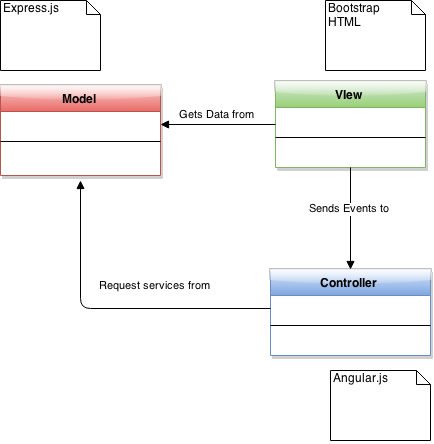
\includegraphics[width=0.5\textwidth]{MVC}}
	    	\caption{Model View Controller}
	    	\label{fig:Learning rate 0.1}
   	\end{figure}
	The purpose of the MVC is to decouple the entities from each other. This will allow us to build Phonegap apps out of our client side. Each component can the evolve on its own through the development phase. 
	The properties of the MVC that we want to take advantage of is as follows.
	\begin{itemize}
		\item Simplification through separation of concerns.
		\item Reuse of the view components.
		\item Maintainability, that facilitates the development by different team members.
		\item Testability as testing is a crucial part of our design and thus this has a great influence.
	\end{itemize}
\end{itemize}